%
% File acl2019.tex
%
%% Based on the style files for ACL 2018, NAACL 2018/19, which were
%% Based on the style files for ACL-2015, with some improvements
%%  taken from the NAACL-2016 style
%% Based on the style files for ACL-2014, which were, in turn,
%% based on ACL-2013, ACL-2012, ACL-2011, ACL-2010, ACL-IJCNLP-2009,
%% EACL-2009, IJCNLP-2008...
%% Based on the style files for EACL 2006 by
%%e.agirre@ehu.es or Sergi.Balari@uab.es
%% and that of ACL 08 by Joakim Nivre and Noah Smith

\documentclass[11pt,a4paper]{article}
\usepackage[hyperref]{acl2019}
\usepackage{times}
\usepackage{latexsym}
\usepackage{verbatim}
\usepackage{url}
\usepackage{fixltx2e}
\usepackage{graphicx}

\aclfinalcopy % Uncomment this line for the final submission
%\def\aclpaperid{***} %  Enter the acl Paper ID here

%\setlength\titlebox{5cm}
% You can expand the titlebox if you need extra space
% to show all the authors. Please do not make the titlebox
% smaller than 5cm (the original size); we will check this
% in the camera-ready version and ask you to change it back.

\newcommand\BibTeX{B\textsc{ib}\TeX}

\title{COMTRAVO-DS team at GermEval 2019 shared task on hierarchical classification of blurbs}

\author{David S. Batista \\
  Comtravo GmbH \\
  {\tt david.batista@comtravo.com} \\\And
  Matti Lyra \\
  Comtravo GmbH \\
  {\tt matti.lyra@comtravo.com} \\}


\date{}

\begin{document}
\maketitle
\begin{abstract}
\textbf{TODO:}
\ \newline
\end{abstract}


\section{Introduction}

This paper describes the approach taken for the GermEval'19 task 1 taken by the Comtravo data-science team.
The task aimed at developing systems to tackle the task of multi-label hierachical classifiction of text.
We took two distinct approaches, one based on a local classifier strategy, where different classifiers are
trained according to the hierarchical structure of the label space. The second


This paper is organized as follows, in Section~\ref{task} we describe task in detail and give a
description of the dataset provided. In Section~\ref{hierarchical-clf} we describe some of the
proposed approaches in the literature to performer hierarchical document classification.
In Section~\ref{system} we describe the system we build to tackle the task and the approaches taken.
Section~\ref{experiments} details the experiments done and the results, finally in
Section~\ref{future} we outline some future work and ideas.

\section{Task}\label{task}

The GermEval 2010 Shared Task on hierarchical classification of blurbs challenges involved the
classification of books into genres given a book's blurb i.e., a short textual description of the
book. The competition contained two sub-tasks:

\begin{itemize}

\item Sub-Task A: classify German books into one or multiple most general writing genres. Therefore,
it can be considered a multi-label classification task. In total, there are 8 classes that can be
assigned to a book.

\item Sub-Task B: targets hierarchical multi-label classification into multiple writing genres. In
addition to the very general writing genres, additional genres of different specificity can
be assigned to a book.

\end{itemize}


\subsection{Dataset}

The dataset made available for this task contains 3 levels and it's considered a hierarchically
multi-label since any example can be can assigned to more than one class at any given level of
the hierarchy. The hierarchy contains a total of 343 classes distinct classes, and in overall there
are 16 627 samples available for training. Table~\ref{quantitivy-analysis-train} as a detailed statistical
description of the dataset.

% every child has exacly one parent, The underlying hierarchy is a forest.

% hierarchy-tree
% imbalence of classes ?
% taxonomy or tree ?
% Whether the taxonomy is organized into a tree or a DAG influences the degree of difficulty of
% the underlying hierarchical classification problem

\begin{table}
\small
\begin{center}
\begin{tabular}{|l|r|}
\hline\centering\textbf{Training dataset}  &                    \\
\hline
Avg. lenght of blurb (tokens)              &  96.78             \\
Std. deviation $\sigma$ (tokens)           &  39.63             \\
Avg. lenght of blurb (sentences)           &  6.55              \\
Std. deviation $\sigma$ (sentences)        &  2.76              \\
\hline
Total number of genres                     &  343               \\
Possible genres per level (1;2;3)          &  8; 93; 242        \\
Avg. genres per per blurb                  &  3.1               \\
Std. deviation $\sigma$                    &  1.36              \\
Avg. genres per blurb at level (1;2;3)     &  1.06; 1.34; 0.69  \\
Std. deviation $\sigma$                    &  0.27; 0.76; 0.79  \\
\hline
Avg. blurb per co-occurrence               &  6.48              \\
Co-Occurrence std. deviation               & 35.90              \\
\hline
Nr. samples with leaf nodes at:            &                    \\
 - Level 1                                 & 1.9\% (311)        \\
 - Level 2                                 & 44,6\% (7.422)     \\
 - Level 3                                 & 53,5\% (8.894)     \\
\hline
\end{tabular}
\end{center}
\caption{\label{quantitivy-analysis-train}Quantitative analysis of the training dataset.}
\end{table}


\begin{table}
\small
\begin{center}
\begin{tabular}{|l|r|}
\hline\centering\textbf{Development dataset}  &             \\
\hline
Avg. lenght of blurb (tokens)              &   98.71        \\
Std. deviation $\sigma$ (tokens)           &   46.29        \\
Avg. lenght of blurb (sentences)           &   6.68         \\
Std. deviation $\sigma$ (sentences)        &   3.80         \\
\hline
Total number of genres                     &                 \\
Possible genres per level (1;2;3)          &          \\
Avg. genres per per blurb                  &                 \\
Std. deviation $\sigma$                    &                \\
Avg. genres per blurb at level (1;2;3)     &    \\
Std. deviation $\sigma$                    &    \\
\hline
Avg. blurb per co-occurrence               &                \\
Co-Occurrence std. deviation               &               \\
\hline
Nr. samples with leaf nodes at:            &                    \\
 - Level 1                                 &         \\
 - Level 2                                 &      \\
 - Level 3                                 &      \\
\hline
\end{tabular}
\end{center}
\caption{\label{quantitivy-analysis-train}Quantitative analysis of the development dataset.}
\end{table}


\begin{comment}

Genres
======

Avg. genres per label 3.114959114959115
Std. deviation :  1.3987352962695292

Avg. genres per label per level
Level  0
1.0726310726310726
0.27751189660762704

Level  1
1.3516113516113517
0.8018182243230956

Level  2
0.6907166907166907
0.7946315397653263

Avg. blurb per co-occurrence
3.08
8.194562864126715

Leaf nodes at each level (1;2;3)
1 : 34 0.016354016354016353
2 : 932 0.4482924482924483
3 : 1113 0.5353535353535354
\end{comment}






\begin{table}
\begin{center}
\begin{tabular}{|l|r|}
\hline\centering\textbf{Test dataset}  &         \\
\hline
Avg. lenght of blurb (tokens)              &  96.91             \\
Std. deviation $\sigma$ (tokens)           &  39.83             \\
Avg. lenght of blurb (sentences)           &  6.55              \\
Std. deviation $\sigma$ (sentences)        &  2.62              \\
\hline
\end{tabular}
\end{center}
\caption{\label{quantitivy-analysis-dev}Quantitative analysis of the test dataset.}
\end{table}


% TODO: grafico com histogram de freqs. para tokens/sentence/genre ?
% TODO: Avg. blurb per co-occurrence ?


\section{Hierarchical Classification}\label{hierarchical-clf}


\ \newline
\textbf{TODO:}
\ \newline


\subsection{Local Classifier}

The local classifier strategy is one way to approach the hierarchical document classification task
and it was first proposed, to the best of our knowledge, in the seminal work of Koller and
Sahami~\shortcite{Koller:1997:HCD:645526.657130}, it is also sometimes referred to as top-down
approach in the literature.

There are different approaches, based on the idea of a local classifier, depending on how they use
the local information and devise a strategy to build several classifiers~\cite{Silla:2011:SHC:1937796.1937884}.


\subsubsection{A classifier per node} % Local Classifier Per Node Approach
The \textit{local classifier per node approach} consists in training one binary classifier for each
node in the hierarchy tree, where a node is every possible label in the hierarchy tree.

For instance, having classes 1, 2 and 3 in the first level, one classifier can be trained with
samples belonging to class 1 as positive and classes 2 and 3 as negative, a similar approach is then
followed for the the other classes and lower levels in the hierarchy. There are different strategies
on how to select the positive and negative classes (see~\cite{}).

During prediction a top-down strategy is applied, the output of each binary classifier will be a
prediction of whether or not a given test sample belongs to the classifier’s predicted class. This
approach is naturally multi-label since it is possible to predict multiple labels per class level.

This approach however is prone to class-membership inconsistency, consider having again in the first
level classes 1, 2 and 3, and in the second level, for instance, classes 1.1, 1.2, since the
classifiers for nodes 1 and 1.1 are independently trained, one can classify a sample as belonging to
classes 1.2 and 1.1 but not to class 1. This approach should also be complemented by a
post-processing method that tries to correct the prediction inconsistency.


\subsubsection{A classifier per parent node} % Local Classifier Per Parent Node Approach
In \textit{a per parent node approach}, for each parent node in the hierarchy tree, a multi-class
classifier is trained to classify the probability of a given sample belonging to each of the parent's
child nodes. A parent node is in this case every label in the hierarchy-tree which has one or more
child labels.

Given a test sample, first the top-level classifier is applied, then for every top-level
predicted class (e.g., class 2 and 3) we apply it's child classifiers, e.g.: a classifier
trained to predicted every 2.x classes and another for 3.x classes, and so one until we reach the
last level.

Note that the sub-classifiers were trained only with the children of classes 2 and 3, therefore
this approach avoids the problem of making inconsistent predictions and respects the constrains
of class-membership defined by the hierarchy-tree.


\subsubsection{A classifier per level} % Local Classifier Per Level Approach
The \textit{local classifier per level} approach consists of training one multi-class classifier
for each level of the hierarchy-tree. When a new test sample is presented we get the output of the
classifiers from each level and use this information as the final classification.

This approach however is prone to class-membership inconsistency, since different classifiers are
trained for each level of the hierarchy. For instance, it's possible to have has outputs for the
first-level classes 2 and 3, and then classes 1.1 and 1.2 at the second-level, and class 3.1.1
at the third-level, which generates an inconsistent classification. This approach should also
be complemented by a post-processing method that tries to correct the prediction inconsistency.

One common error to all strategies in the local classifier and the top-down class-prediction
approach is the propagation of errors downwards the hierarchy.



\subsection{Global Classifier: labels co-occurrence}

Another type of strategy is to learn a classifier than can globally learn to output the predictions
for each level in the hierarchical structure. This is done by flatenning and hierarchical structure
and leveraging on the labels co-occurrence.

\citet{kurata-etal-2016-improved} proposed a novel neural network initialisation method to
treat some of the neurons in the final hidden layer as dedicated neurons for each pattern of label
co-occurrence These dedicated neurons are initialised to connect to the corresponding co-occurring
labels with stronger weights than to others.


\begin{comment}
When the labels form a hierarchy, they share a hypernym–hyponym relation. When multiple
 labels are assigned to the text, if it is explicitly labeled by a subclass it must also implicitly
 include all of the its super- classes.
The co-occurrence between subclasses and superclasses as labels for the input text contains
information we would like to leverage to improve multi-label classification using a neural network.
\end{comment}








\section{System}\label{system}

In our developed system we tried out two main approaches: a classifier per
parent node (parent-node), and global classifier by exploring the
labels co-occurrence.



\subsection{Local Classifier}

We employed a parent per parent approach, which has the advantage of not being
prone to hierarchy inconsistency errors. We need to train classifiers for
parents node, so we for the Level 3 we don't need to train any classifier
since it contains only leaf nodes, plus some nodes on Level 2 are already leaf
nodes.

According to Table~\ref{quantitivy-analysis-train} the first level has 8 possible
labels, which means that the parent node of the first level (i.e, the Root node)
needs to be trained in a multi-label fashion and predict over 8 classes. Each of
these 8 classes represents a parent node of some child classes on then
second level of the hierarchy. So for Level 1 we need to train eight multi-label
classifiers where the labels are the child`s of each parent in the root level.
Finally, for Level 2, we train 42 classifiers only, since according to the
hierarchy-tree some labels in this level are already leaf nodes. In total we
trained 51 classifiers distributed by different levels as described in
Table~\ref{parent-per-node-classifiers}.

\begin{table}[!h]
\begin{center}
\begin{tabular}{|l|r|}
\hline\centering\textbf{Level}  &  \textbf{Nr. Parent Nodes}    \\
\hline
Root              &  1       \\
Level 1           &  8       \\
Level 2           &  42      \\
\hline
Total Classifiers & 51       \\
\hline
\end{tabular}
\end{center}
\caption{\label{parent-per-node-classifiers}Number of parent nodes per level in the hierarchy.}
\end{table}

\subsection{Global Classifier}



\ \newline
\textbf{TODO:}
\ \newline


\begin{figure}[h]
\centering
    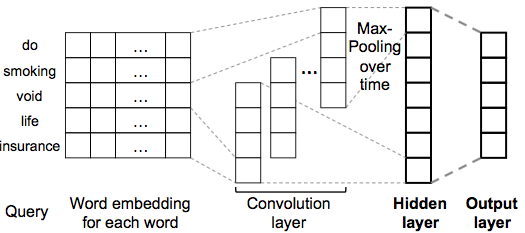
\includegraphics[width=8cm]{global_classifier_nn.png}
    \caption{Convolutional Neural Networks for sentence classification with weight initialization. (adapted from )}
    \label{fig:mesh1}
\end{figure}


\begin{figure}[h]
    \centering
    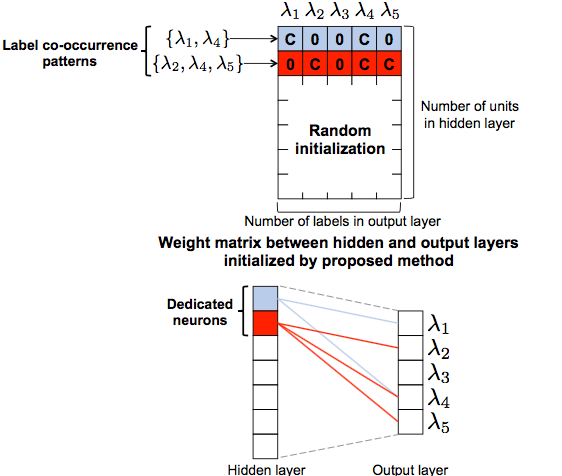
\includegraphics[width=8cm]{global_classifier_init.png}
    \caption{Weight initialization matrix (adapted from )}
    \label{fig:mesh1}
\end{figure}




\section{Experiments and Results}\label{experiments}

\ \newline
\textbf{TODO:}
\ \newline

\subsection{Results on the Development Set}

We randomly split the development data into training (70\%) and test (30\%) sets.
The training set was used to develop and trained classifiers, and the test set
to evaluate the trained classifiers.

\subsubsection{Local classifier per node: root classifier}

The best results were achieved with the following classifiers configuration.

For the root node we trained a logistic regression with TF-IDF weighted vectors
in a one-versus-rest scenario using the scikit-learn 0.21.1~\cite{Pedregosa:2011:SML:1953048.2078195}.

% class_weight='balanced', solver='sag', max_iter=50000
% The "balanced" mode uses the values of y to automatically adjust weights inversely proportional to
% class frequencies in the input data as ``n_samples / (n_classes * np.bincount(y))``.

We pre-processed the data by first tokenising the blurbs into sentences, and then
from sentences into tokens. We consider the title of the book a sentence. We used
the german sentence tokeniser, and the \textit {word\_punkt\_tokenizer} both available
on NLTLK 3.4.1~\cite{Bird:2009:NLP:1717171}, also, we only considered alphanumeric
tokens, i.e., all punctuation tokens were discarded.

% What else did we tried? % de_stemmer = GermanStemmer() % stop-words ?

We preformed a parameter search, on 3 folds over the training set, varying following parameters:

\begin{itemize}
\item token n-grams: \{(1), (1,2),(1,3)\}
\item token lowercase: \{True, False\}
\item norm: \{l1, l2\}
\item regularization C: \{0.1, 10, 100, 300\}
\end{itemize}

This classifier is also the one that reports the results for Sub-Task A. We also experimented with
other methods for the root classifier, namely with: Hierarchical Attention Networks~(HAN)~\cite{yang-etal-2016-hierarchical},
Bag-of-Tricks~\cite{joulin-etal-2017-bag}, bi-LSTM~\cite{Hochreiter:1997:LSM:1246443.1246450}, ConvNets~\cite{kim-2014-convolutional}


\begin{table}
\begin{center}
\begin{tabular}{|l|r|r|r|}
\hline\centering\textbf{Method}  & \textbf{Precision} &  \textbf{Recall} &  \textbf{F\textsubscript{1}}\\
\hline
 ConvNets       & 0.8635 & 0.8000 & 0.8305 \\
 Logit (TF-IDF) & 0.8216 & 0.8363 & 0.8289 \\
 HAN            & 0.8101 & 0.7574 & 0.7829 \\
 bi-LSTM        & 0.8016 & 0.7031 & 0.7492 \\
 Bag-of-Tricks  & 0.5325 & 0.4964 & 0.5138 \\

\hline
\end{tabular}
\end{center}
\caption{\label{devset-results} Results for different classifiers on the Sub-Task A}
\end{table}

\subsubsection{Local classifier per node: 1st and 2nd levels}

For Level 1 and 2 in the hierarchy tree we trained classifiers based the convolutional
neural networks sentence classification model from~\citet{kim-2014-convolutional}.

We implemented the variation of the proposed architecture based on pre-trained embeddings
which are fine-tuned during learning, and we used the public available German fastText embeddings
trained on Wikipedia, of dimension 300 and obtained using the skip-gram model described in
~\citet{bojanowski-etal-2017-enriching} with default parameters.

We used rectified linear units in the activation functions of the 1D convolutions,
filter windows (i.e., n-grams) of size 1 and 2 with 300 feature maps each and a
dropout rate of 0.5.

Training is done with the Adam optimizer~\cite{journals/corr/KingmaB14} over
shuffled mini-batches of size 16 for 10 epochs and using 33\% of the data for validation.
The neural network was implemented in Keras 2.2.4 with Tensorflow 1.13.1 backend.

% TODO: advantages and disadvantages of this method?


We then applied the best classifiers and parameters on the dev set and run the evaluation.
Table~\ref{devset-results} shows the results for both tasks with the system described above on the
development set.

\begin{table}
\begin{center}
\begin{tabular}{|l|r|r|r|}
\hline\centering\textbf{Task}  & \textbf{Precision} &  \textbf{Recall} &  \textbf{F\textsubscript{1}}\\
\hline
 Sub-Task A   & 0.8247 & 0.8291 & 0.8269 \\
 Sub-Task B   & 0.6930 & 0.5602 & 0.6196 \\
\hline
\end{tabular}
\end{center}
\caption{\label{devset-results} Best achieved results on the development set for both Sub-Tasks A and B.}
\end{table}









\subsection{Official Results}

\ \newline
\textbf{TODO:}
\ \newline

\section{Future Work}\label{future}

% other features, release date, author's name


\ \newline
\textbf{TODO:}
\ \newline




\section*{Acknowledgments}

\ \newline
\newpage
\bibliography{konvens2019.bib}
\bibliographystyle{acl_natbib}

\begin{comment}

\appendix

\section{Appendices}
\label{sec:appendix}
Appendices are material that can be read, and include lemmas, formulas, proofs, and tables that are not critical to the reading and understanding of the paper.
Appendices should be \textbf{uploaded as supplementary material} when submitting the paper for review. Upon acceptance, the appendices come after the references, as shown here. Use
\verb|\appendix| before any appendix section to switch the section
numbering over to letters.


\section{Supplemental Material}
\label{sec:supplemental}
Submissions may include non-readable supplementary material used in the work and described in the paper. Any accompanying software and/or data should include licenses and documentation of research review as appropriate. Supplementary material may report preprocessing decisions, model parameters, and other details necessary for the replication of the experiments reported in the paper. Seemingly small preprocessing decisions can sometimes make a large difference in performance, so it is crucial to record such decisions to precisely characterize state-of-the-art methods.

Nonetheless, supplementary material should be supplementary (rather
than central) to the paper. \textbf{Submissions that misuse the supplementary
material may be rejected without review.}
Supplementary material may include explanations or details
of proofs or derivations that do not fit into the paper, lists of
features or feature templates, sample inputs and outputs for a system,
pseudo-code or source code, and data. (Source code and data should
be separate uploads, rather than part of the paper).

The paper should not rely on the supplementary material: while the paper
may refer to and cite the supplementary material and the supplementary material will be available to the
reviewers, they will not be asked to review the
supplementary material.
\end{comment}

\end{document}
